\section[Electromagnetically Induced Transparency in $\Lambda$-Type Atoms]
  {Electromagnetically Induced Transparency\\ in $\Lambda$-Type Atoms}
  \label{sec:polaritons_eit}

    We recall from section \ref{sec:nonlinear_threelevel} that the
    $\Lambda$-configuration three-level atom consists of two lower states
    $\Ket{0}$ and $\Ket{2}$ coupled to a single excited state $\Ket{1}$.
    Transitions between the two lower states are dipole forbidden.

    We apply a probe field near-resonant with the $\Ket{0}$ to $\Ket{1}$
    transition and a strong coupling field on the $\Ket{2}$ to $\Ket{1}$
    transition. The total electric field in the slowly varying envelope
    approximation (see section \ref{sec:propagation_deriving}) is given by 
    \begin{equation}
      \mathbf{E}(z,t) = \left[ \tfrac{1}{2} \mathbf{\hat{x}}_p 
        \mathcal{E}_p(z,t) \ee^{\ii(k_p z - \omega_p t)} + 
        \tfrac{1}{2} \mathbf{\hat{x}}_c \mathcal{E}_c(z,t) \ee^{\ii(k_c z -
        \omega_c t)} + \cc \right]
      \label{eqn:lambda_field}
    \end{equation}
   where $\mathbf{\hat{x}}_p$ and $\mathbf{\hat{x}}_c$ are orthogonal
    polarisation of the vectors of the fields and the envelopes $\mathcal{E}_p$
    and $\mathcal{E}_c$ are in general complex functions. We define
    corresponding Rabi frequencies $\Omega_p = d_{01}\mathcal{E}_p/\hbar$ and
    $\Omega_c = d_{21}\mathcal{E}_c/\hbar$ where $d_{j1}$ is the dipole moment
    between levels $\Ket{j}$ and $\Ket{1}$, which we take parallel to its
    respective field polarisation.

    We then find the Hamiltonian for the $\Lambda$ system interacting with this
    pair of classical fields to be\cite{Fleischhauer2005}
    \begin{equation}
      \mathcal{H}_\mathrm{\Lambda} = -\hbar \left[ \Delta_p \sigma_{11} + 
        (\Delta_p - \Delta_c) \sigma_{22} \right] - \hbar \left[ \Omega_p 
        \sigma_{10} + \Omega_c \sigma_{12} + \hc \right]
      \label{eqn:lamda_hamiltonian}
    \end{equation}
    within the dipole approximation and in the frame rotating with the
    frequencies of the optical fields. Here $\sigma_{ij} := \Ket{i}\Bra{j}$ is
    the transition operator.

    If we write out the components of the Lindblad master equation (equation
    \ref{eqn:lindblad}) we obtain a set of differential equations for the
    density matrix elements

    \begin{subequations}
    \begin{align}
      \frac{\partial \rho_{00}}{\partial t} &= \Gamma_{10} \rho_{11} + 
      \frac{\ii}{\hbar} \left[ \Omega_p \rho_{10} - \cc \right] \\
      %%
      \frac{\partial \rho_{01}}{\partial t} &= - \left(\ii \Delta_p + 
      \tfrac{\Gamma_{10}}{2} \right) \rho_{01} - \ii \rho_{01} \Omega^*_p 
      \left( \rho_{00} - \rho_{11} \right) - \ii \Omega^*_c \rho_{02} \\
      %%
      \frac{\partial \rho_{02}}{\partial t} &= \left( - 
      \ii (\Delta_p - \Delta_c) - \tfrac{\Gamma_{20}}{2} \right) \rho_{02} + 
      \ii \Omega^*_p \rho_{12} - \ii \Omega_c \rho_{01} \\
      %%
      \frac{\partial \rho_{11}}{\partial t} &= -(\Gamma_{10} + \Gamma_{12}) 
      \rho_{11} + \frac{\ii}{\hbar} \left[ \Omega_p \rho_{01} - \cc \right] + 
      \ii \left[ \Omega_c \rho_{21} - \cc \right] \\
      %%
      \frac{\partial \rho_{12}}{\partial t} &= \left(\ii \Delta_c - 
      \tfrac{\Gamma_{12}}{2} \right) \rho_{12} + \ii \Omega_p \rho_{02} + 
      \ii \Omega_c \left( \rho_{22} - \rho_{11} \right) \\
      %%
      \frac{\partial \rho_{22}}{\partial t} &= \Gamma_{12} \rho_{11} + 
      \ii \left[ \Omega^*_c \rho_{12} - \cc \right]
    \end{align}
    \label{eqn:lambda_dm_equations}
    \end{subequations}
    Note that $\rho_{10} = \rho_{01}^\dagger$, $\rho_{20} = \rho_{02}^\dagger$
    and $\rho_{21} =\rho_{12}^\dagger$.

  \subsection{Weak Probe Lineshape}

    Now we'll take the same approach we took with the two-level atom in section
    \ref{sec:propagation_twolevel} to look at the optical response in the case
    that the probe field is weak while the coupling field remains strong. We
    assume that the coupling field is turned on long before the weak probe so
    that all population is optically pumped to the ground state $\Ket{0}$ via
    decay from the excited state $\Ket{1}$.

    If we take equation (\ref{eqn:lambda_dm_equations}e) with the time-
    derivative set to zero (\ie the steady state) and neglect the small
    $\Omega_p$, we find
    \begin{equation}
      \rho_{02} = \frac{\Omega_c}{\Delta_p - \Delta_c 
      - \ii \tfrac{\Gamma_{20}}{2}}.
    \end{equation}
    Substituting this into equation (\ref{eqn:lambda_dm_equations}d) and setting
    $\rho_{00} = 1$, we find the following expression for the steady state
    coherence on the probe transition
    \begin{equation}
      \rho_{01} = - \frac{\Omega_p}{\Delta_p + \ii \tfrac{\Gamma_{10}}{2} - 
      \frac{\left| \Omega_c \right|^2 }{\Delta_p - \Delta_c - 
      \ii \tfrac{\Gamma_{20}}{2}}}
    \end{equation}
    which gives us the frequency-dependent susceptibility of the medium to the
    weak probe field in the strongly coupled system. As we expect, setting
    $\Omega_c = 0$ gives us back the two-level lineshape equation
    (\ref{eqn:weak_lineshape}).

    In figure \ref{fig:autler_townes} we show the lineshapes calculated by
    solving the steady-state Lindblad equations --- \ie setting the time
    derivatives in equations (\ref{eqn:lambda_dm_equations}) to zero. We see
    that the effect of the strong coupling field is to split the resonance peak
    by $\Omega_c$. This is the Autler-Townes splitting\cite{Autler1955}. The
    probe coherence $\Im \left[ \rho_{01} \right]$ is, in contrast to the 
    two-level lineshape, zero on resonance, and as we know from equation
    (\ref{eqn:beer_law}) that this is proportional to the absorption, we have a
    frequency window around resonance in which light incident on the medium will
    not be absorbed.

    \begin{figure}[h]
      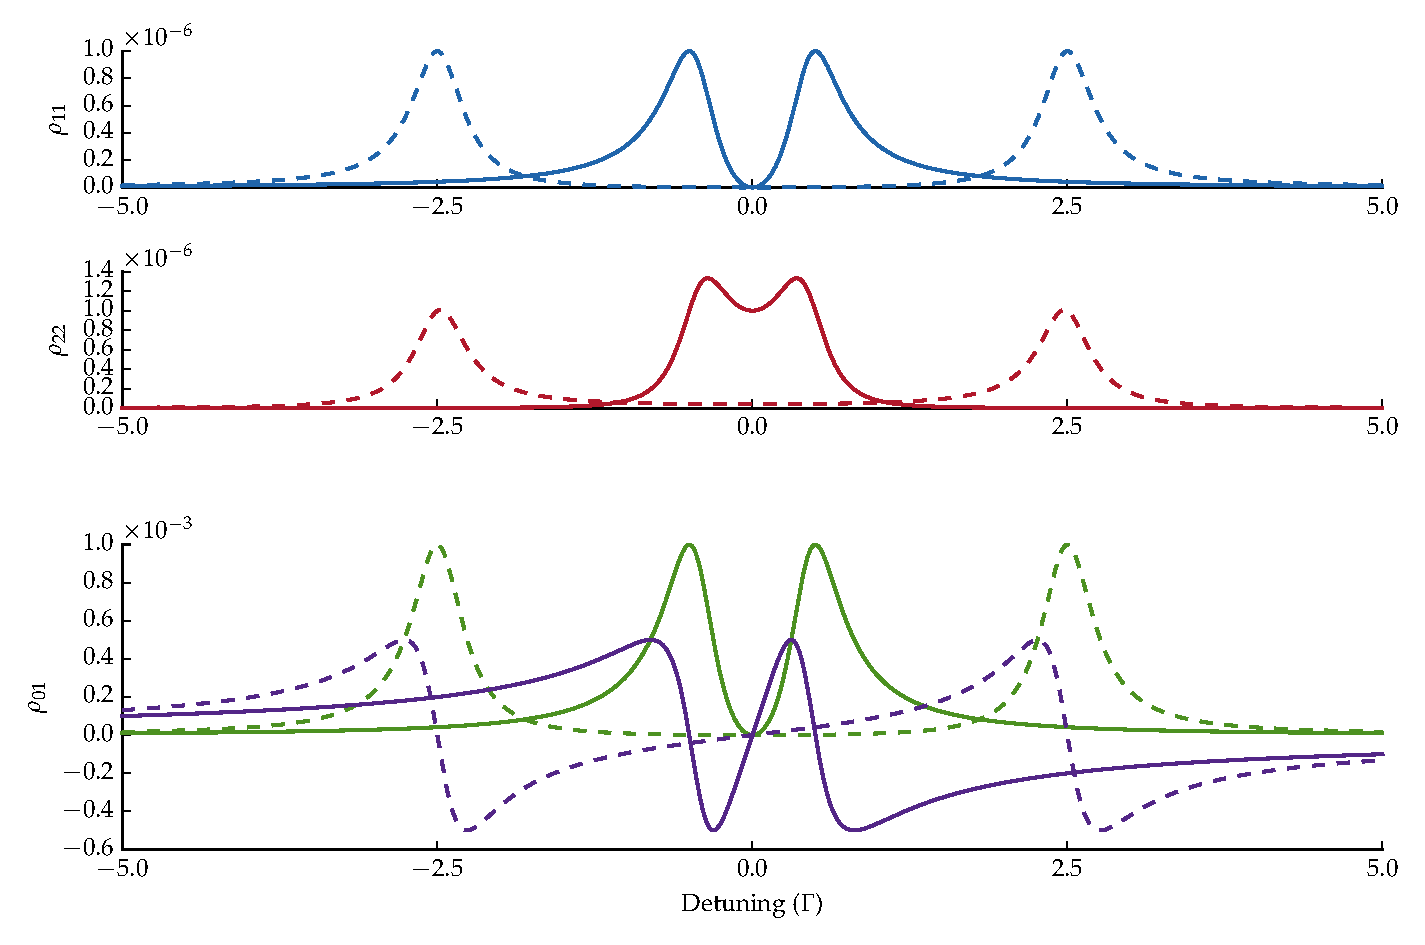
\includegraphics[width=\linewidth]
        {figs/04_polaritons/plot_steady_scan_p000_1_c1_c5_fig1.pdf}
      \caption{
      %%
      Steady-state values for density matrix elements against probe detuning for
      the $\Lambda$ system, with $\Omega_p =
      \unit[2\pi~\times~10^{-3}]{\Gamma_{01}}$. For the solid line $\Omega_c =
      \unit[2\pi~\times~1]{\Gamma_{01}}$, for the dashed line $\Omega_c =
      \unit[2\pi~\times~5]{\Gamma_{01}}$, both on resonance. (Top, blue) The
      excited state population $\rho_{11}$. (Middle, red) The coupled lower
      state population $\rho_{22}$. (Bottom, purple) The real part of the
      coherence  $\Re \left[ \rho_{01} \right]$. (Bottom, green) The imaginary
      part of the coherence  $\Im \left[ \rho_{01} \right]$.
      %%  
      }
      \label{fig:autler_townes}
    \end{figure}

    In figure \ref{fig:autler_townes_narrow} we show the same lineshapes with a
    smaller coupling field Rabi frequency $\Omega_c$. Even then we see a narrow
    window on resonance. This absorption window is the effect known as
    electromagnetically induced transparency (\textsc{eit}). Though objectively
    separating observations of Autler-Townes splitting from \textsc{eit} in
    experiment can be difficult\cite{Anisimov2011}, they are distinguished in
    that only \textsc{eit} provides strong transparency for a weak coupling
    field due to the Fano interference.\cite{Fano1961}

    \begin{figure}[h]
      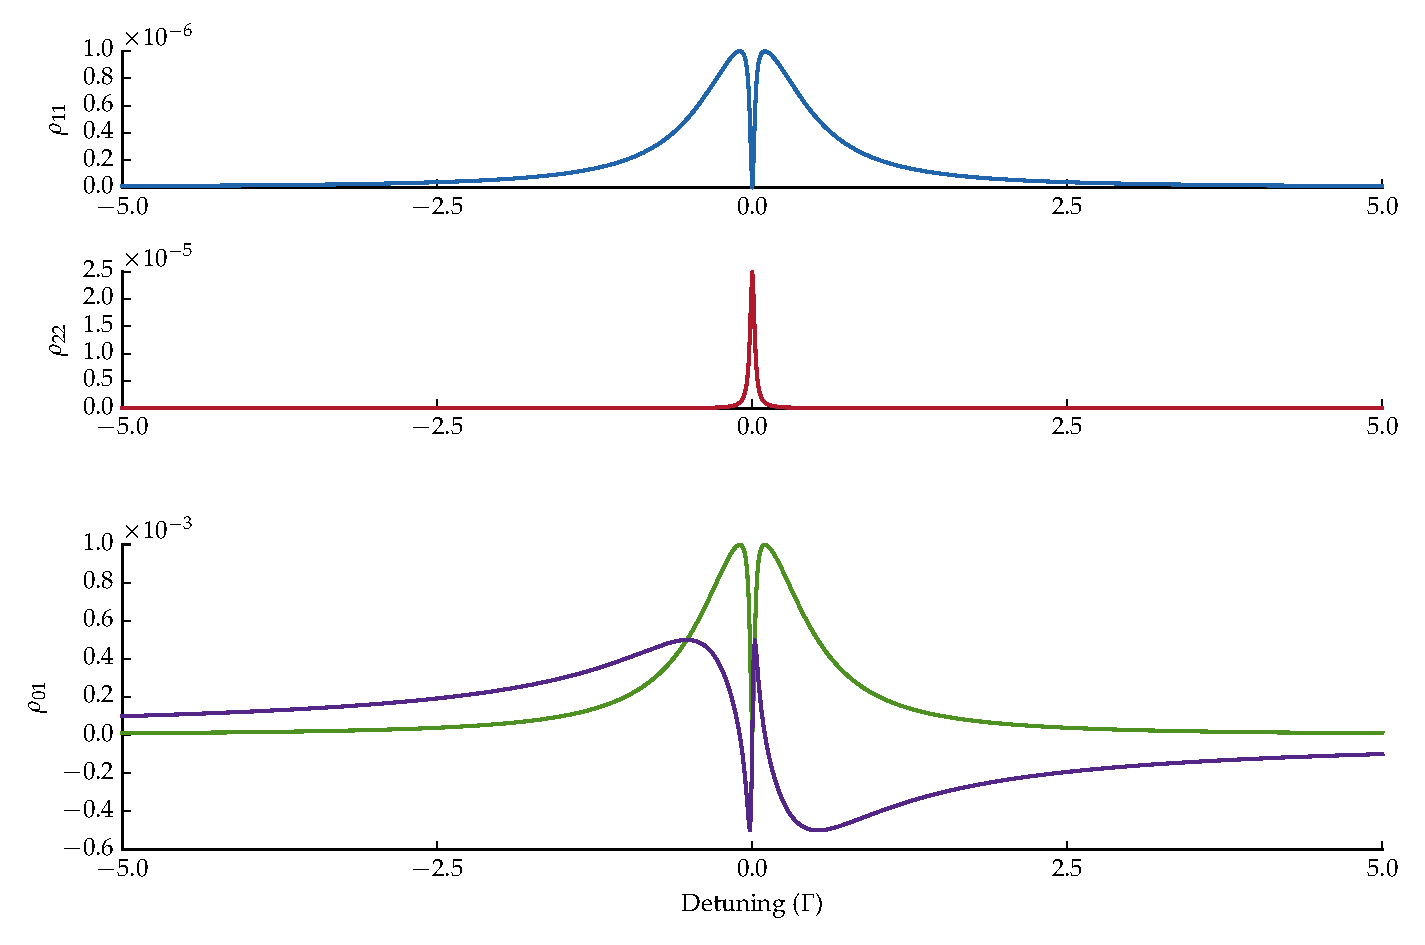
\includegraphics[width=\linewidth]
        {figs/04_polaritons/steady_scan_p000_1_c0_2_fig1.pdf}
      \caption{
      Steady-state values for density matrix elements against probe detuning for
      the $\Lambda$ system, with $\Omega_p =
      \unit[2\pi~\times~10^{-3}]{\Gamma_{01}}$ and $\Omega_c =
      \unit[2\pi~\times~0.2]{\Gamma_{01}}$. (Top, blue) The excited state
      population $\rho_{11}$. (Middle, red) The coupled lower state population
      $\rho_{22}$. (Bottom, purple) The real part of the coherence  $\Re \left[
      \rho_{01} \right]$. (Bottom, green) The imaginary part of the coherence
      $\Im \left[ \rho_{01} \right]$.
      }
      \label{fig:autler_townes_narrow}
    \end{figure}

  \subsection{Coherent Population Trapping \& the Dark State}

    To investigate the cause of this transparency effect, we write the
    Hamiltonian in the so-called coherent population trapping (\textsc{cpt})
    basis by taking the eigenstates of $\mathcal{H}_\Lambda$. Following
    Fleischhauer \etal\cite{Fleischhauer2005}, we solve for $\mathcal{H}_\Lambda
    \Ket{\phi} = \lambda \Ket{\phi}$ with equal detunings $\Delta := \Delta_p =
    \Delta_c$ to find eigenvalues
    \begin{subequations}
      \begin{align}
      \lambda_0 &= 0 \\
      \lambda_\pm &= \pm \bar{\Omega} -\Delta/2 
      \end{align}
      \label{eqn:lambda_eigvals}
    \end{subequations}
    where $\bar{\Omega}= \sqrt{\Omega_p^2 + \Omega_c^2 + \Delta^2}$. The
    eigenvalues have corresponding normalised eigenstates 
    \begin{subequations}
      \begin{align}
        \Ket{D} &= \frac{1}{\sqrt{N_0}} \big( \Omega_c \Ket{0} - \Omega_p 
        \Ket{2} \big) \\
        \Ket{B_\pm} &= \frac{1}{\sqrt{N_\pm}} \big( \Omega_p \Ket{0} + 
          \lambda_\pm \Ket{1} + \Omega_c \Ket{2} \big)
      \end{align}
      \label{eqn:lambda_eigvects}
    \end{subequations}
    where $N_0 := \Omega_p^2 + \Omega_c^2$ and $N_\pm := N_0 + 4 \lambda_\pm^2$.
    The first thing to notice is that the $\lambda_0$ energy eigenvalue is zero
    such that it is decoupled from the fields. Second, its corresponding
    eigenstate $\Ket{D}$ has no component of the excited state $\Ket{1}$ and so
    population in this \textit{dark state} has no opportunity to decay to either
    of the lower states. The probe laser then couples only to the $\Ket{1}$
    components of the bright states $\Ket{B_\pm}$ having equal magnitude but
    opposite contributions such that we end up with destructive interference of
    excitation and the probe laser is not absorbed. We thus see that
    \textsc{eit} is a quantal coherent phenomenon.

    

    % [TODO write a sentence on experimental observation, Harris]

    % \cite{Harris1990, Boller1991}